\section{Gaussian Process Model}\label{sec:gpmodel}

GP can be applied as probabilistic models to regression problems. Here we use the GP model to generalise a stellar model grid to a continuous and probabilistic function that maps inputs to observable quantities. 
%
As mentioned in Section~\ref{sec:grid}, our model grid has four independent fundamental inputs, i.e., mass, initial metallicity, initial helium fraction, and mixing-length parameter. Adding the {\it EEP} which describes the evolutionary phase, the GP model contents five inputs. We intend to train GP models that predict effective temperature, surface gravity, radius, surface metallicity, and stellar age. We summary GP model inputs and outputs as below.
\begin{itemize}
\item GP model inputs and their dynamic ranges:
\item[] Mass ($M$ = 0.8 -- 1.2$\rm M_{\odot}$)
\item[] Equivalent Evolutionary Phase ({\it EEP} = 0 -- 1)
\item[] Initial metallicity ([Fe/H]$_{\rm init}$ =  -0.5 -- 0.5 dex)
\item[] Initial helium fraction ($Y_{\rm init}$ = 0.24 -- 0.32)
\item[] Mixing-length parameter ($\alpha_{\rm MLT}$ = 1.7 -- 2.5)
\item GPR model outputs: 
\item[] Effective temperature ($T_{\rm eff}$) 
\item[] Surface gravity ($\log g$)
\item[] Radius ($R$)
%\item[] The large spacing ($\Delta\nu$)  
\item[] Surface metallicity ([Fe/H]$_{\rm surf}$)
\item[] Stellar age ($\tau$)
\end{itemize}
We aim to use the GP model as a non-parametric emulator, that is emulating the comparatively slow calls to models of stellar evolution.
This emulator can be described as
\begin{equation}\label{gprmodel}
{\rm Outputs} = f(M, EEP, ({\rm Fe/H})_{\rm init}, Y_{\rm init}, \alpha_{\rm MLT}). 
\end{equation}


\subsection{Gaussian Process Application}

In our application to grids of stellar models,  a GP has a number of desirable properties.  While a GP is a stochastic process, the distribution of a GP can be considered as a distribution of functions with a continuous domain.  In fact,  the marginal likelihood considered in function space is equal to the likelihood of the data given some function values,  multiplied by the prior on those function values marginalised over all function values \cite{williams1996gaussian}.  That is to say that, the GP allows for the analytical evaluation of a fit over many different functions (perhaps an infinite number) weighted by some concept of a prior and the agreement with the data.   In addition,  while the marginal likelihood will be assessed on discrete data,  predictions can be made using linear algebra for new data in the continuous domain, but crucially again marginalised over these many different functional forms.  It is possible to see how this might be useful for generalising (or emulating or augmenting) a discrete grid of stellar models in order to obtain predictions in the continuous domain.

In this section we will look at the required mathematics to be able to implement a GP for our application to grids of stellar models.  We start with a series of definitions before dealing with the marginal likelihood and the posterior predictive distributions. 

We start with a grid of stellar models containing $N$ models with a label we want to learn, for example model effective temperature, which we will denote with the general symbol $\bf y$, and a set of input labels $\bf X$ (e.g., mass, age, and metallicity).  We can use a GP to make predictions of the effective temperature (labelled $y$) for additional input values given by $\bf X_{\star}$.  The vector $\bf y$ is arranged ${\bf y} = \left(y_{i}, ... ,y_{N} \right)^{T}$ where the subscript label references the stellar model.  The input labels are arranged into a $N \times D$ matrix where $D$ is the number of input dimensions (e.g., $D=3$ for mass, age, and metallicity) so that ${\bf X} = ({\bf x}_{1}, ..., {\bf x}_{N})^{T}$ where ${\bf x_{i}} = (x_{1, i}, ..., x_{D, i})^{T}$.  The matrix of additional inputs $\bf X_{\star}$ has the same form as $\bf X$ but size $N_{\star} \times D$.

\citet{williams1996gaussian}, from which our description below is based,  define a GP as a collection of random variables, where any finite number of which have a joint Gaussian distribution.  In general terms,  a GP may be written so that our labels are random variables drawn from our GP distribution, 
\begin{equation}
{\bf y}({\bf x}) \sim \mathcal{GP}\left( m({\bf x}),  k({\bf x}, {\bf x'})\right),
\end{equation}
where $m({\bf x})$ is some mean function, and $k({\bf x}, {\bf x'})$ is some covariance function that could generate the covariance matrix $\bf \Sigma$.  The mean function controls the deterministic part of the regression and the covariance function controls the stochastic part.  The mean function defined here could be any deterministic function and we will label the additional parameters, or hyperparameters, $\phi$.  Each element of the more familiar covariance matrix is defined by the covariance function or {\it kernel function} $k$ which has hyperparameters $\theta$ and is given by,
\begin{equation}
{\bf \Sigma}_{n, m} = k({\bf x}_{n}, {\bf x}_{m},  \theta),
\end{equation}
where the inputs ${\bf x}_{i}$ are $D$-dimensional vectors and the output is a scalar covariance.

{\bf Tanda - does Gpy use a white noise term here too? }

{\bf Guy, there is a white noise in the likelihood function and it is a free parameter. As mentioned in section 3.2.2, 'this noise parameter is set as free and it reduces to a small value in the training progress.'}

\subsubsection{The likelihood}
Conceptually we value the GP because of it's ability to marginalise over many functions $\bf f$ and return a marginal likelihood,
\begin{equation}
p({\bf y} | {\bf X}) = \int p({\bf y} | {\bf f}, {\bf X}) p({\bf f} | {\bf X}) \, {\rm d}{\bf f}.
\end{equation}
This integral could be evaluated.  However, by noting that a GP is a collection of random variables, where any finite number of which have a joint Gaussian distribution, the marginal probability of our data $\bf y$ is also the joint likelihood of a multivariate normal distribution,
\begin{equation}
p({\bf y} | {\bf X}) = \mathcal{N}(m({\bf X}), {\bf \Sigma}),
\end{equation}
which can be straightforward to evaluate.  Thus the marginal log likelihood ... 

{\bf TODO : add equation}

{\bf TODO : Comment on O() for det and inverse}

\subsubsection{Making predictions}
If we want to obtain predictive distributions for the output $\bf y_{\star}$ given the inputs $\bf X_{\star}$ the joint probability distribution of $\bf y$ and $\bf y_{\star}$ is Gaussian and given by
\begin{equation}
p \left( \begin{bmatrix} {\bf y} \\ {\bf y_{\star}} \end{bmatrix} \right) = \mathcal{N} \left( \begin{bmatrix} m({\bf X}) \\ m({\bf X_{\star}}) \end{bmatrix} , \begin{bmatrix} {\bf \Sigma} & {\bf K_{\star} }\\ {\bf K_{\star}}^{T} & {\bf K_{\star \star}} \end{bmatrix}  \right), 
\end{equation}
where the covariance matrices $\bf \Sigma$ and $\bf K$ are computed using the kernel function so that

{\bf Guy- can we name $\bf \Sigma$ and $\bf K$ in some way? I feel that a name helps readers to remember what the parameter is.}

\begin{equation}
{\bf \Sigma}_{n, m} = k({\bf X}_{n}, \, {\bf X}_{m}),
\end{equation}
which is an $N \times N$ matrix.
\begin{equation}
{\bf K}_{\star \, n, m} = k({\bf X}_{n}, \, { \bf X}_{\star \, m}),
\end{equation}
which is an $N \times N_{\star}$ matrix, and finally
\begin{equation}
{\bf K}_{\star \star \, n, m} = k({\bf X}_{\star \, n},  {\bf X}_{\star \,m}),
\end{equation}
which is an $N_{\star} \times N_{\star}$ matrix.
The predictions of $\bf y_{\star}$ are again a Gaussian distribution so that,
\begin{equation}
{\bf y}_{\star} \sim \mathcal{N}(\bf \hat{y}_{\star}, \, \bf C),
\label{eq:pred}
\end{equation}
where 
\begin{equation}
{\bf \hat{y}}_{\star} = m({\bf X}_{\star}) + {\bf K}_{\star}^{T} \, {\bf \Sigma}^{-1} \, ({\bf y} - m(\bf X)),
\end{equation}
and 
\begin{equation}
{\bf C} = {\bf K}_{\star \star} - {\bf K}_{\star}^{T} \, {\bf \Sigma}^{-1} \, {\bf K_{\star}}.
\end{equation}

At point we can make predictions on model properties given a grid of stellar models using equation \ref{eq:pred}.  But these predictions will be poor unless we select sensible values for the form and hyperparameters of the mean function and covariance function.  In the following section we detail a number of kernel functions that will be tested against the data.  We will then discuss the method for determining the values of the hyperparameters to be used.


\subsection{Setting up the GP Model}\label{sec:set_up}

We adopt a tool package named \textsc{GPyTorch}, which is a GP framework developed by \citet{gardner2018gpytorch}. It is a Gaussian process library based on an open source machine-learning framework PyTorch (\url{https://pytorch.org}). The package provides significant GPU acceleration, state-of-the-art implementations of the latest algorithmic advances for scalability and flexibility, and easy integration with deep learning frameworks. Source codes and detailed introductions could be found on \url{https://gpytorch.ai}.

For training GP models, we need set up mean function, kernel function, likelihood function, loss function, and optimiser. 
To find out the best option for each of above elements, we do a number of preliminary tests. 
These tests are carried out with 2-demission (2D) GP models which map $M$ and {\it EEP} to the five observable outputs (Outputs = $f(M, EEP)$). Training data are selected from the primary grid with fixed [Fe/H]$_{\rm init}$ (0.0), $Y_{\rm init}$ (0.28), and $\alpha_{\rm MLT}$ (2.1). There are 41 evolutionary tracks which content 24,257 data points. We also compute 44 evolutionary tracks with the same [Fe/H]$_{\rm init}$, $Y_{\rm init}$, and $\alpha_{\rm MLT}$ but random $M$ for the purpose of validating and testing. We use the method mentioned in Section \ref{sec:selection} and sample 20,000 data points for training, 10,000 for validating, and 10,000 for testing. 
%
We start with the \textsc{Simple GP Regression} example (\url{https://docs.gpytorch.ai/en/stable/examples/01_Exact_GPs/Simple_GP_Regression.html}) and develop our own method step by step as follow. 

\subsubsection{Mean Function}

We first investigate the mean function. As discussed above, the data distribution is generally smooth but complex in sub-areas. Although a GP model does not significantly affected by the choice of mean function because of the flexibility of kernels, we find that using a constant or a linear mean function leads to a long time for training. For this reason, we apply a Neural Network mean function which is flexible enough to manage both simple and complex features. We adopt an architecture including 6 hidden layers and 128 nodes per layer. All layers apply the linear transformation to the incoming data. We apply the element-wise function (Elu) because it give relatively smooth mean functions. ({\bf Can Guy or Alex add some references for NN and Elu here? The referee may ask why the 6x128 architecture is sufficient, so should we mention Alex's paper?})

\subsubsection{Likelihood and Loss Function}

We then work on the likelihood function and the loss function. Our training object is a theoretical model grid. There is hence no observed uncertainty for each data point, but a tiny random uncertainty exists due to the approximations in the \textsc{MESA} numerical method. The noise model can be assumed as a Gaussian function with a very small deviation. 
%   
A likelihood specifies the mapping from latent function values $f(X)$ to observed labels $y$.
We adopt the the standard likelihood for regression which assumes a standard homoskedastic noise model whose conditional distribution is
\begin{equation}\label{eq:likelihood}
p(y|f(x)) = f + \epsilon, \epsilon \sim \mathcal{N}(0, \sigma^{2}),
\end{equation}
where $\sigma$ is a noise parameter. 
%
We use a small and fixed noise parameter and run a few tests. However, the strict noise parameter makes GP models hard to converge. When this noise parameter is set as free, it reduces to a small value anyway in the training progress because it is data-driven. For this reason, we decide not put strict constraint for or prioritise this noise parameter. In practice, we only set up a loose upper limit ($\sigma$  < 0.1) to speed up the training. One thing should be noted that a GP model with a large noise parameter is not a proper description for the stellar grid. Because of this, we only adopt GP models with $\sigma$ $\lesssim 10^{-4}$.   
The loss function is simply the exact marginal likelihood in the logarithmic scale.

\subsubsection{Optimiser}

Afterwards, we study the optimiser. We mainly compare between two optimiser named SGD and Adam. Here SGD refers to Stochastic Gradient Descent, and Adam is a combination of the advantages of two other extensions of stochastic gradient descent, specifically, Adaptive Gradient Algorithm and Root Mean Square Propagation. 
%
The SGD optimiser in the \textsc{GPyTroch} package involves the formula given by \citet{sutskever2013importance}. The formula makes it possible to train using stochastic gradient descent with momentum thanks to a well-designed random initialisation and a particular type of slowly increasing schedule for the momentum parameter. The application of momentum in SGD could improve its efficiency and make it less likely to stuck in local minimums. On the other hand, the Adam optimiser includes the 'AMSGrad' variant developed by \citet{47409} to improve its weakness in the convergence to an optimal solution. With these new developments, the two optimisers give very similar results. We finally choose Adam because it works relatively efficiently and stable.  
%
We adaptive learning rate in the training process. Our training starts with a learning rate of 0.01 and decreases by a factor of 2 when the loss value does not reduce in previous 100 iterations.    

\subsubsection{Early Stopping}

We set up an Early Stopping for avoiding overfitting and also determining when to terminate a training progress. 
When an optimal solution is found, the validating errors stop decreasing and then increase when overfitting occurs. 
We hence track down the validating error every iteration and terminate training process when the validating error does not decrease in previous 300 iterations. 	

\subsubsection{Kernel Function}

With the above set up, we test different kernel functions. We involve four basic kernels as listed below:
\begin{itemize}
\item RBF: Radial Basis Function kernel (also known as squared exponential kernel)
\item RQ: Rational Quadratic Kernel (equivalent to adding together many RBF kernels with different lengthscales)
\item Mat12: Matern 1/2 kernel (equivalent to the Exponential Kernel)
\item Mat32: Matern 3/2 kernel 
\end{itemize}
We apply each basic kernel and a couple of combined kernels (RBF + Mat21, RQ + Mat21, Mat32 + Mat21, RBF + Mat32, RQ + Mat32) to train and validate GP model for each output. Among these kernels, the combined kernel RBF+Mat21 gives the best fit to the training data, however, it does not give the best predictions for validating and testing data. On the other hand, the Mat32 kernel fits training data reasonably well and it predicts the best for validating and testing data. 
%
Comparing between the two kernels, the RBF+Mat12 Kernel is a combination of a smooth and a spiky kernel, which has sufficient flexibility to fit features of data. However, the spiky function make it less accurate for off-grid regions. 
%
The smoothness of Mat32 kernel is somewhere between a spiky (Mat21) and a smooth kernel (RBF). It does not exactly fit some sharp features but it maps the off-grid region with better continuity. We hence adopt the Mat32 kernel for the training. 

\subsubsection{Training Procedure}

We lastly introduce the procedure of training a GP model. The full process includes training, validating, and testing. 
In the training process, we literately optimise hyperparameters of a GP model to learn the underline function which maps inputs to outputs from on-grid evolutionary tracks (training dataset). In each iteration, the GP model is validated by comparing true and GP predicted values of off-grid tracks (validating dataset). Although the validating dataset is not directly involved in training hyperparameters, it still constructs the GP model to some extend because the optimal solution is the one that best fits the validating dataset. For this reason, the validating dataset does not give a completely independent validation for a GP model. 
%
We hence have a testing process at the end for the purpose of estimating the systematic uncertainty of GP. We reserve a half of off-grid tracks as testing dataset and qualify a GP model using the testing error (true value - GP prediction).


\section{Preliminary Studies on Low-Demission Problems}\label{examples}

In this section, we present GP applications on 1-, 2-, and 3-demissions (1D, 2D, 3D) problems. We also investigate two key questions before training the 5-demissions (5D) stellar grid: testing method and strategy for large sample. 

\subsection{1D Problem}

We first demonstrate an example of GP application on an 1D problem. We train a GP model to learn the evolution of effective temperature for a $\rm 1.1M_{\odot}$ track. We split the data points on this track into training and testing data by 70-to-30. We train a GP model which maps  {\it EEP} to effective temperatures. We then compare true and GP-predicted effective temperatures of testing data. As it can be seen in Figure \ref{fig:1dgp},  the GP model gives very accurate predictions: residuals are within $\pm$0.5 K. As a comparison, we fit the training data with the quadratic function and use it to predict testing data. We find that the two methods give very similar results. It indicate that GP can be an alternative of classical interpolators on the 1D problem. 

\begin{figure}
	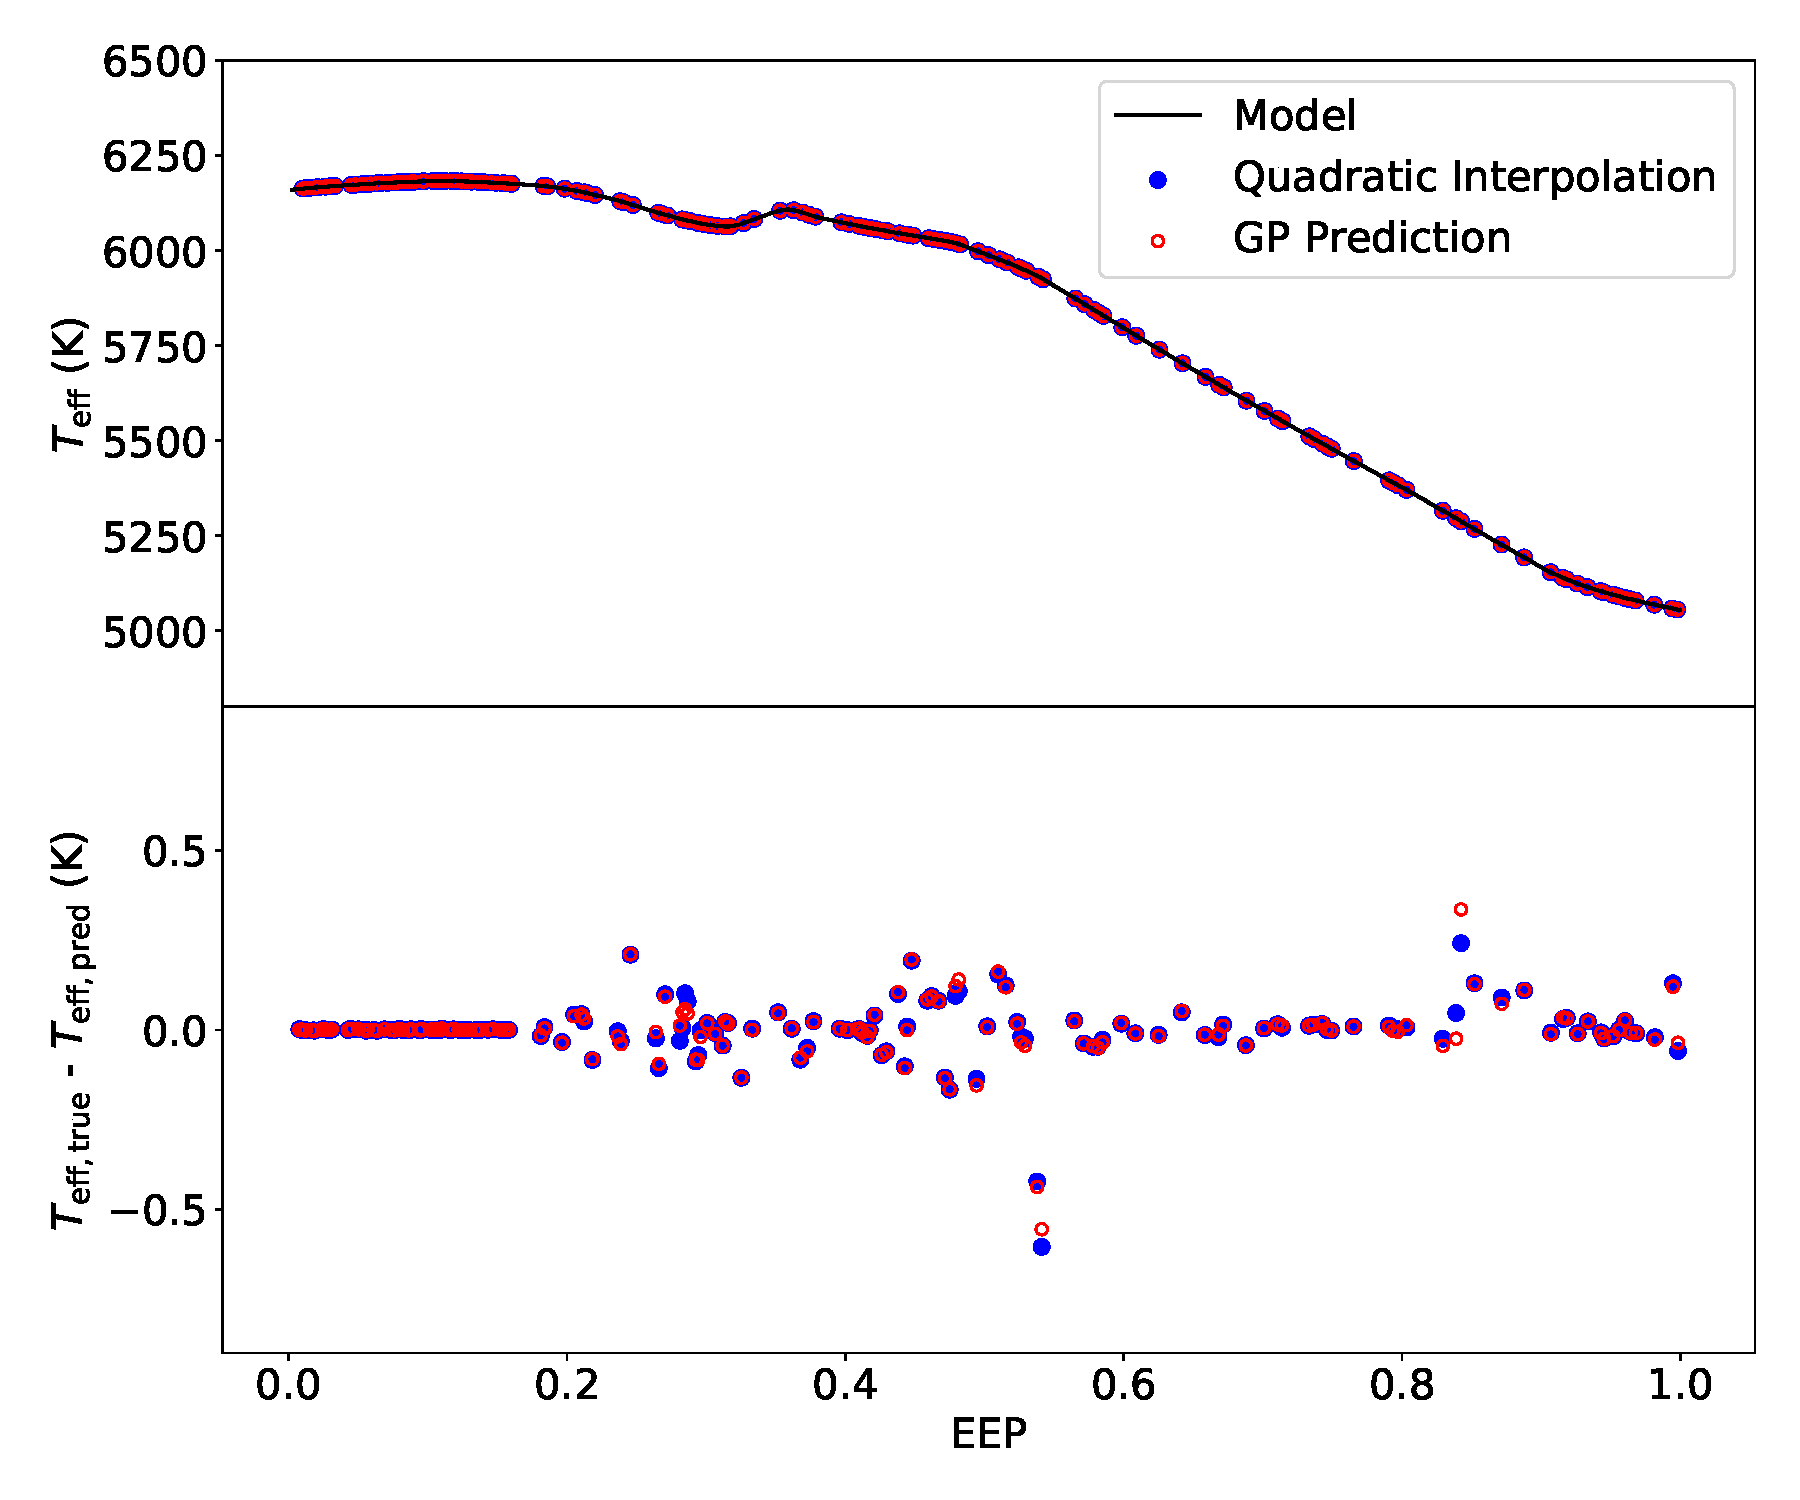
\includegraphics[width=1.0\columnwidth]{1d-gp.pdf}
    \caption{GP application on 1D problem. Models on this track are split into training and testing data by 70-to-30, Top: the evolution of effective temperature for a $\rm 1.1M_{\odot}$ track. The grey line is the evolutionary track computed with \textsc{MESA}; blue and red circles indicate predictions for the testing data from the quadratic interpolator and the GP model. Bottom: residuals of predictions in the top graph. }  
    \label{fig:1dgp}
\end{figure}

\subsection{2D Problem: Investigating testing method}

We present a 2D example here.  We use the same training, validating, and testing datasets mentioned in Section \ref{sec:set_up} and train GP models which map $M$ and {\it EEP} to observables. We illustrate the GP model for effective temperature in Figure \ref{fig:2dtest}. As it shown that, GP transforms the sparse data into a continuous function and hence is able to predict values for unseen points.
%
We also notice that the kernel function in the area of $M \geq 1.05 {\rm M_{\odot}}$ and ${\it EEP} \leq 0.7$ is more complex than that for other regions because of the appearance of the 'hook'. This particular area are relatively difficult to learn and poorly predicted by the GP model. 

\begin{figure}
	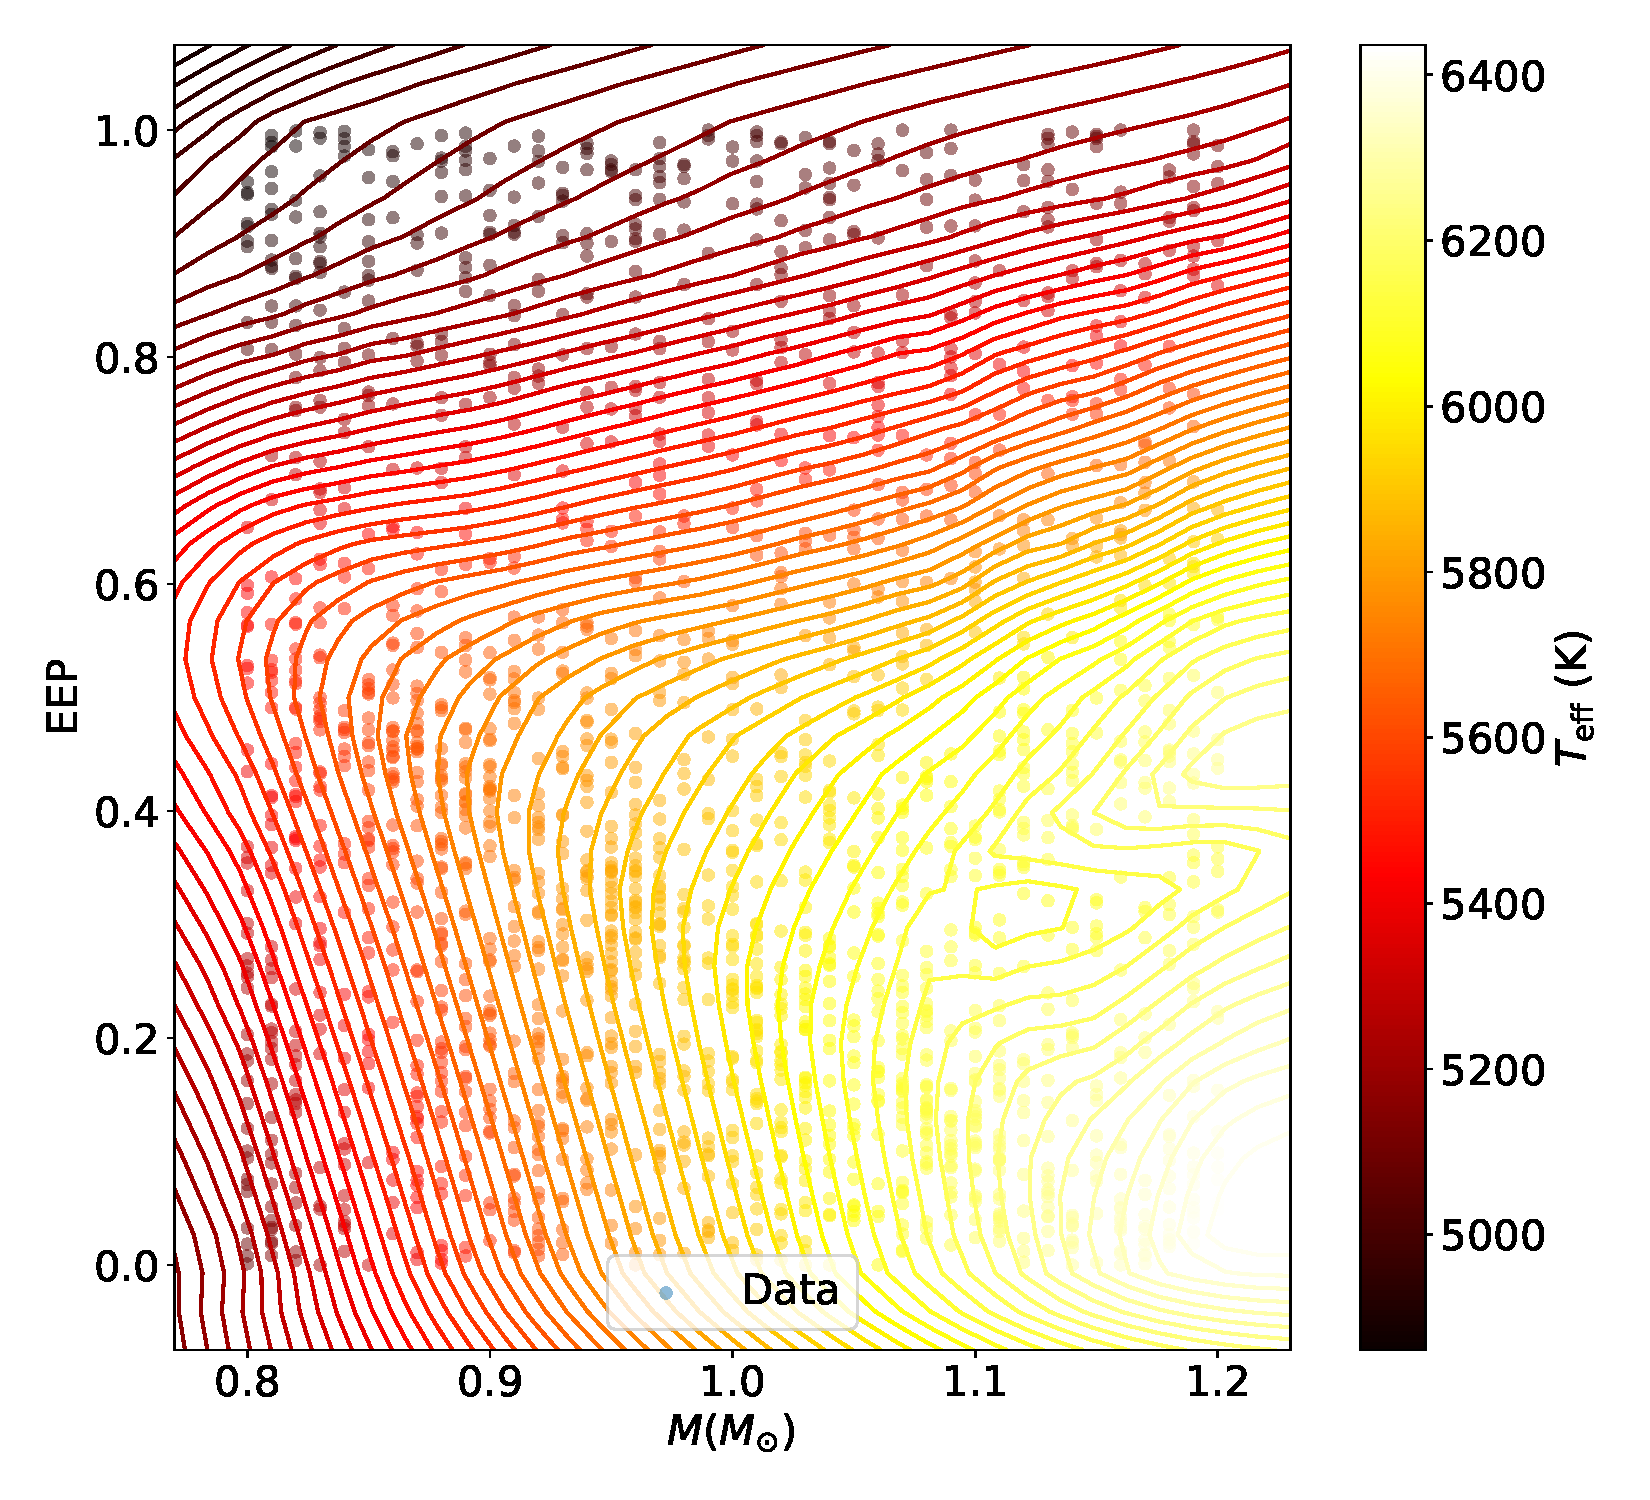
\includegraphics[width=1.0\columnwidth]{2d_GPmodel_function.pdf}
	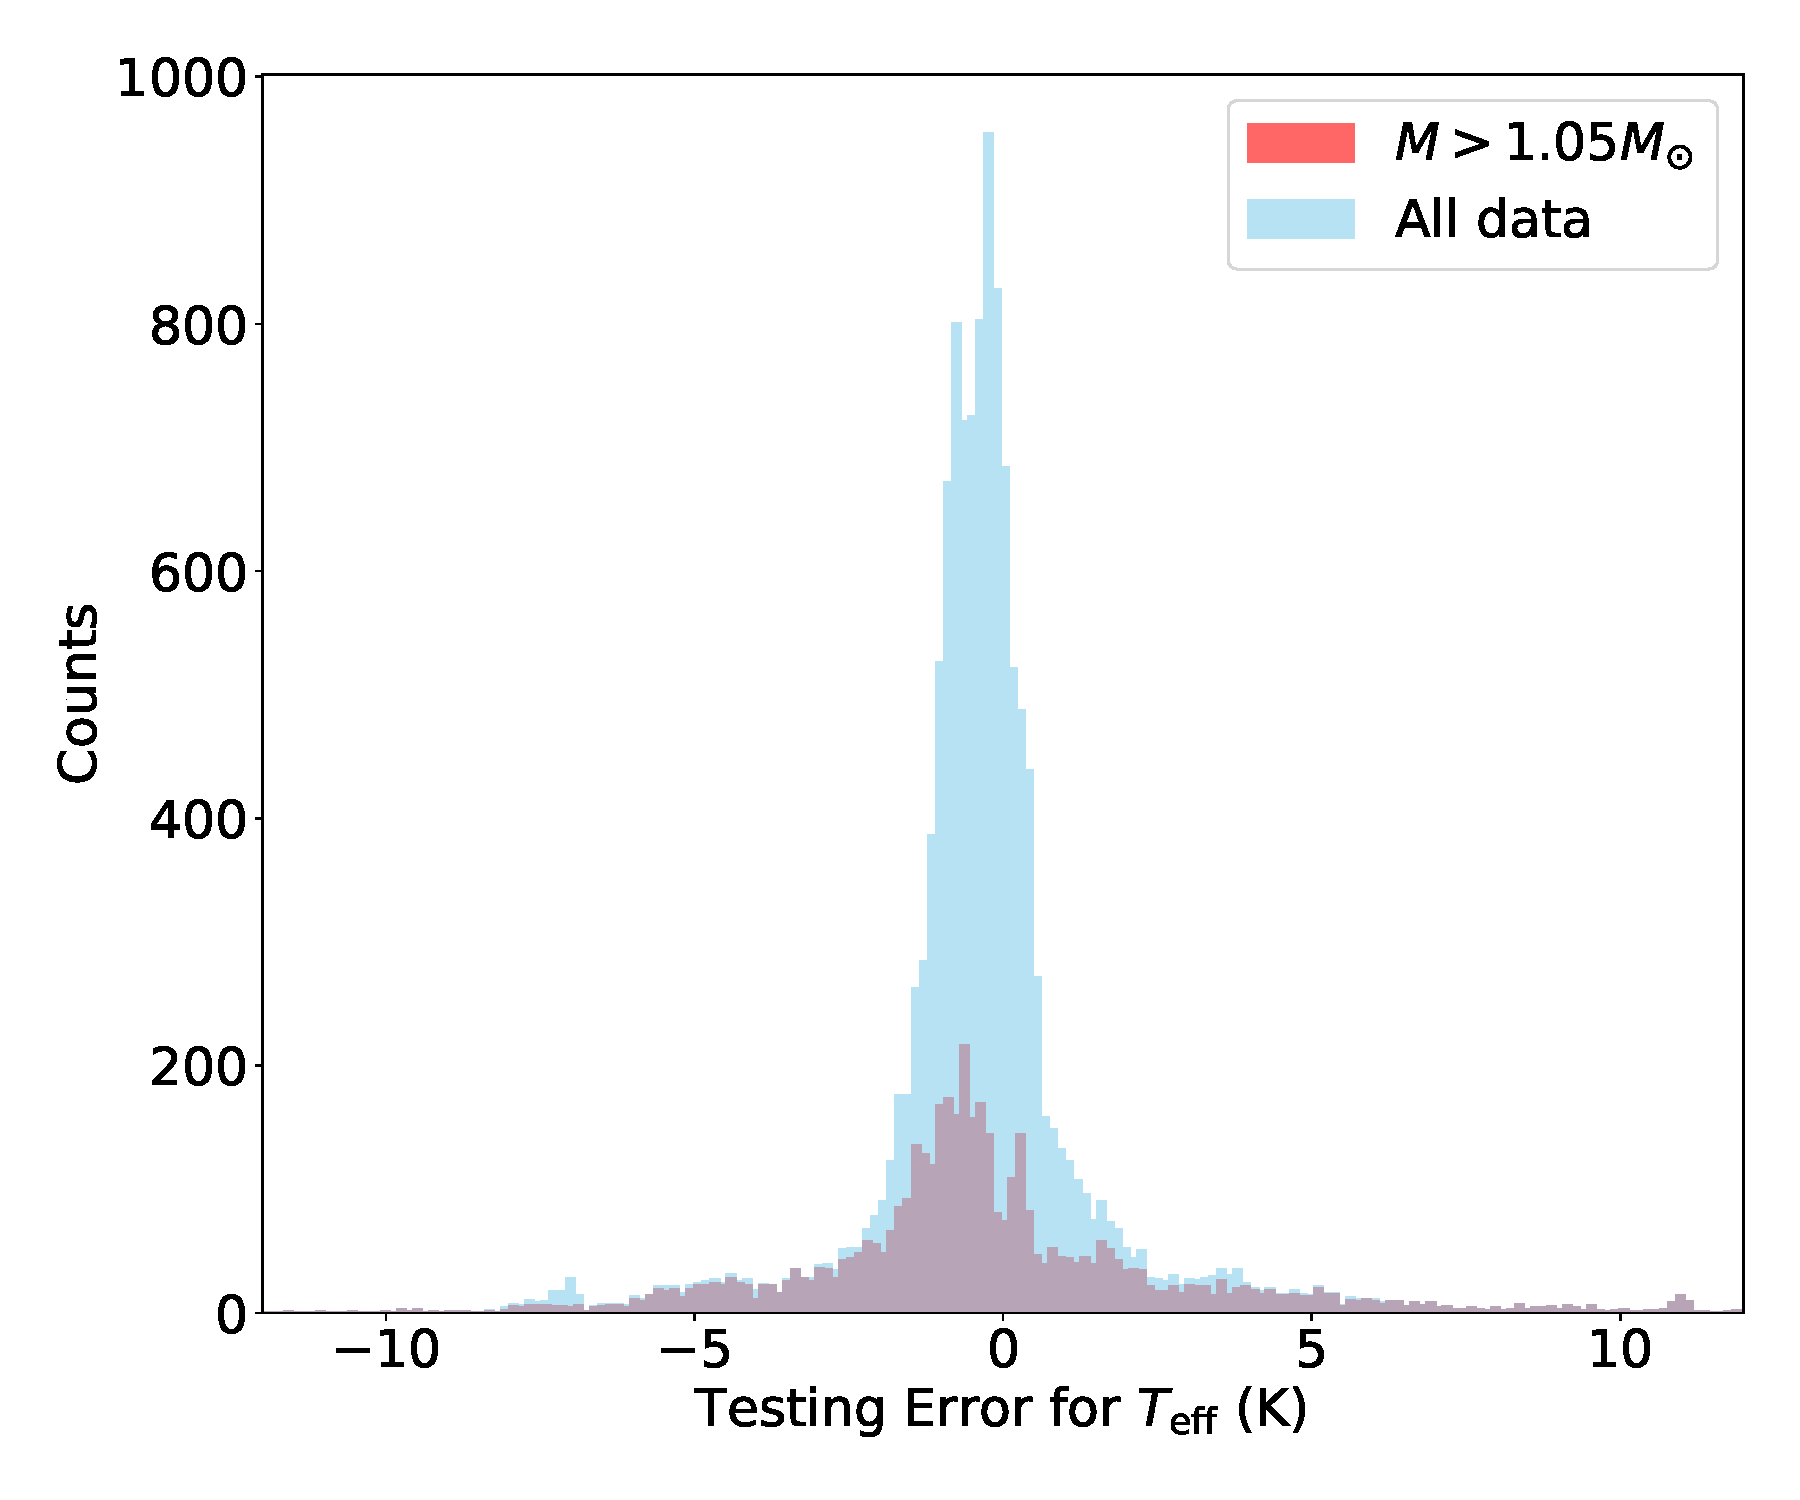
\includegraphics[width=1.0\columnwidth]{2d_testing_hist_effective_T.pdf}	
    \caption{Top: The 2D GP model for $T_{\rm eff}$. Bottom: probability distributions of validating errors of the GP model. }  
    \label{fig:2dtest}
\end{figure}

When there is a subregion in which the GP model performs worse than other areas, the probability distribution of testing error is not quite a  Gaussian function. We examine the error distribution as shown at the bottom of Figure \ref{fig:2dtest}. Errors of most data follows a Gaussian distribution but about $10\%$ data form long tails on both sides. 
%
We inspect testing errors for other output parameters and find similar results. 
The cases of surface gravity and radius are similar to the effective temperature. The surface metallicity is not affected by the hook, but the GP predictions are relatively poor at the early subgiant phase in high-mass tracks. This is because high-mass tracks maintain shallow convective envelope and hence have strong diffusion effect during the main-sequence stage. At the early subgiant phase, the quick expansion of the surface convective envelope brings back the settling heavy elements to the surface, leading to a sharp raise of the surface metallicity. 
%
We also find that the accuracy of age prediction drops down for very old low-mass stellar models. This is because age values vary in a relatively big dynamic range (15 - 50 Gyr) in a small fraction of data points. Poor age resolution causes poor GP predictions.        
This is to say, the tail feature is common for all five outputs. This leads to a question of how to quantity the testing error.

For this case, a global error such like Root Mean Square Error (RMSE) is not ideal to quantify the error. Because it does not well reflect the tail feature. What we need here is a method that reflects the general accuracy level as well as the worst case. 
%
We examine the error distribution of each output and count data points in the tails (outside the 3 times of full width at half maximum). The amount of these data are around 10\% (8 - 12\% for different outputs). 
%
For the majority (90\%) of data points, which from a Gaussian function, the 68\% confidential interval is able to reflect their accuracies. For the worst 10\% of the data, we could use the 95\% and 99.7\% confidential intervals to describe the median value and the length of the tail. Thus, we define an Error Index (EI), which is the sum of 68\%, 95\%, and 99.7\% cumulative values of absolute errors, to qualify GP models. For the case in Figure \ref{fig:2dtest}, cumulative values at 68\%, 95\%, and 99.7\% are 1.1, 4.9, and 11.1K, which give an EI equals to 17.1K. 

\subsection{3D Problem: Strategy for Large Data Sample}

As a further step, we apply GP on a 3D grid and investigate the strategy for large data sample.
The model grid we aim to train contents about 10,000,000 data points, which is much more than the upper limit of data size (20,000) of an \textsc{Exact GP} model. We work on this with 3-demission (3D) GP models, which map $M$, {\it EEP}, and  [Fe/H]$_{\rm init}$ to observable outputs. 
%The 3D GP model can be described as Outputs $ = f(M, EEP, {\rm [Fe/H]_{init}})$. 
We select training data from the primary grid with fixed $Y_{\rm init}$ (0.28), and $\alpha_{\rm MLT}$ (2.1). The training dataset contents $\sim$300,000 data points. For validating and testing purposes, we compute another 174 evolutionary tracks with the same input $Y_{\rm init}$ and $\alpha_{\rm MLT}$ but random $M$ and [Fe/H]$_{\rm init}$. Before proceeding with large sample, we train an \textsc{Exact GP} model using 20,000 training data points as a standard reference. 

We first consider the Stochastic Variational GP (SVGP) approach based on the \textsc{GPyTorch ApproximateGP} module. 
%We train our data based on the SVGP example on \url{https://docs.gpytorch.ai/en/v1.1.1/examples/04_Variational_and_Approximate_GPs/SVGP_Regression_CUDA.html}. 
SVGP is an approximate scheme rely on the use of a series of inducing points which can be selected in the parameter space. It trains using minibatches on the training dataset and build up kernels on the inducing points. Underline principles and detailed descriptions of this approach can be found in \citet{hensman2015scalable}. The advantage of SVGP is the large capacity of sample size. However, the kernel complexities is still limited by the amount of inducing points. 
%
In our tests, we find a practical issue with the SVGP approach. Because a large training sample takes off the memory, we can only use 10,000 inducing points. This is to say, the kernel complexity of the SVGP model is even simpler than the Exact GP model which uses 20,000 data points. As a result, the SVGP model does not show any improvements. For instance, the 68th, 95th, and 99.7th testing errors for $T_{\rm eff}$ are 2.0, 5.8, and 15.7 K (EI = 23.5K) for the \textsc{Exact GP} model and 2.2, 6.8, and 15.1K (error index = 24.1 K) for the SVGP one. Because the evolutionary feature are complex across multiple demissions, what we need here is increasing the kernel complexity. This requires more data points that actually construct the kernel function. For this particular case, the SVGP downgrades the complexity and hence does not improve the results.   

We then investigate another approach designed for large dataset named Structured Kernel Interpolation (SKI GP). SKI GP was introduced by \citet{wilson2015kernel}. It produces kernel approximations for fast computations through kernel interpolation and is a great way to scale a GP up to very large datasets (100,000+ data points).
% We follow the example on \url{https://docs.gpytorch.ai/en/stable/examples/02_Scalable_Exact_GPs/KISSGP_Regression.html} to develop our script. 
We run a few tests to train a 3D SKI GP model with 100, 000 training data. Compare with the \textsc{Exact GP} and SVGP, its testing errors for $T_{\rm eff}$ are slightly improved to 2.0, 6.1, and 14.8K (EI = 22.9K). However, the further test on the 5-demission data is not ideal: a SKI GP model using 100, 000 training data performs much worse than an \textsc{Exact GP} model with only 20,000 training data. The poor behaviour consists with what has been discussed in \citet{wilson2015kernel}. The method poorly scale to data with high dimensions, since the cost of creating the grid grows exponentially in the amount of data. We attempt to make some additional approximations with the \textsc{GpyTorch AdditiveStructureKernel} module. It makes the base kernel to act as one-dimension kernels on each data dimension and the final kernel matrix will be a sum of these 1D kernel matrices. However, the testing errors are not significantly improved.

 \begin{figure}
	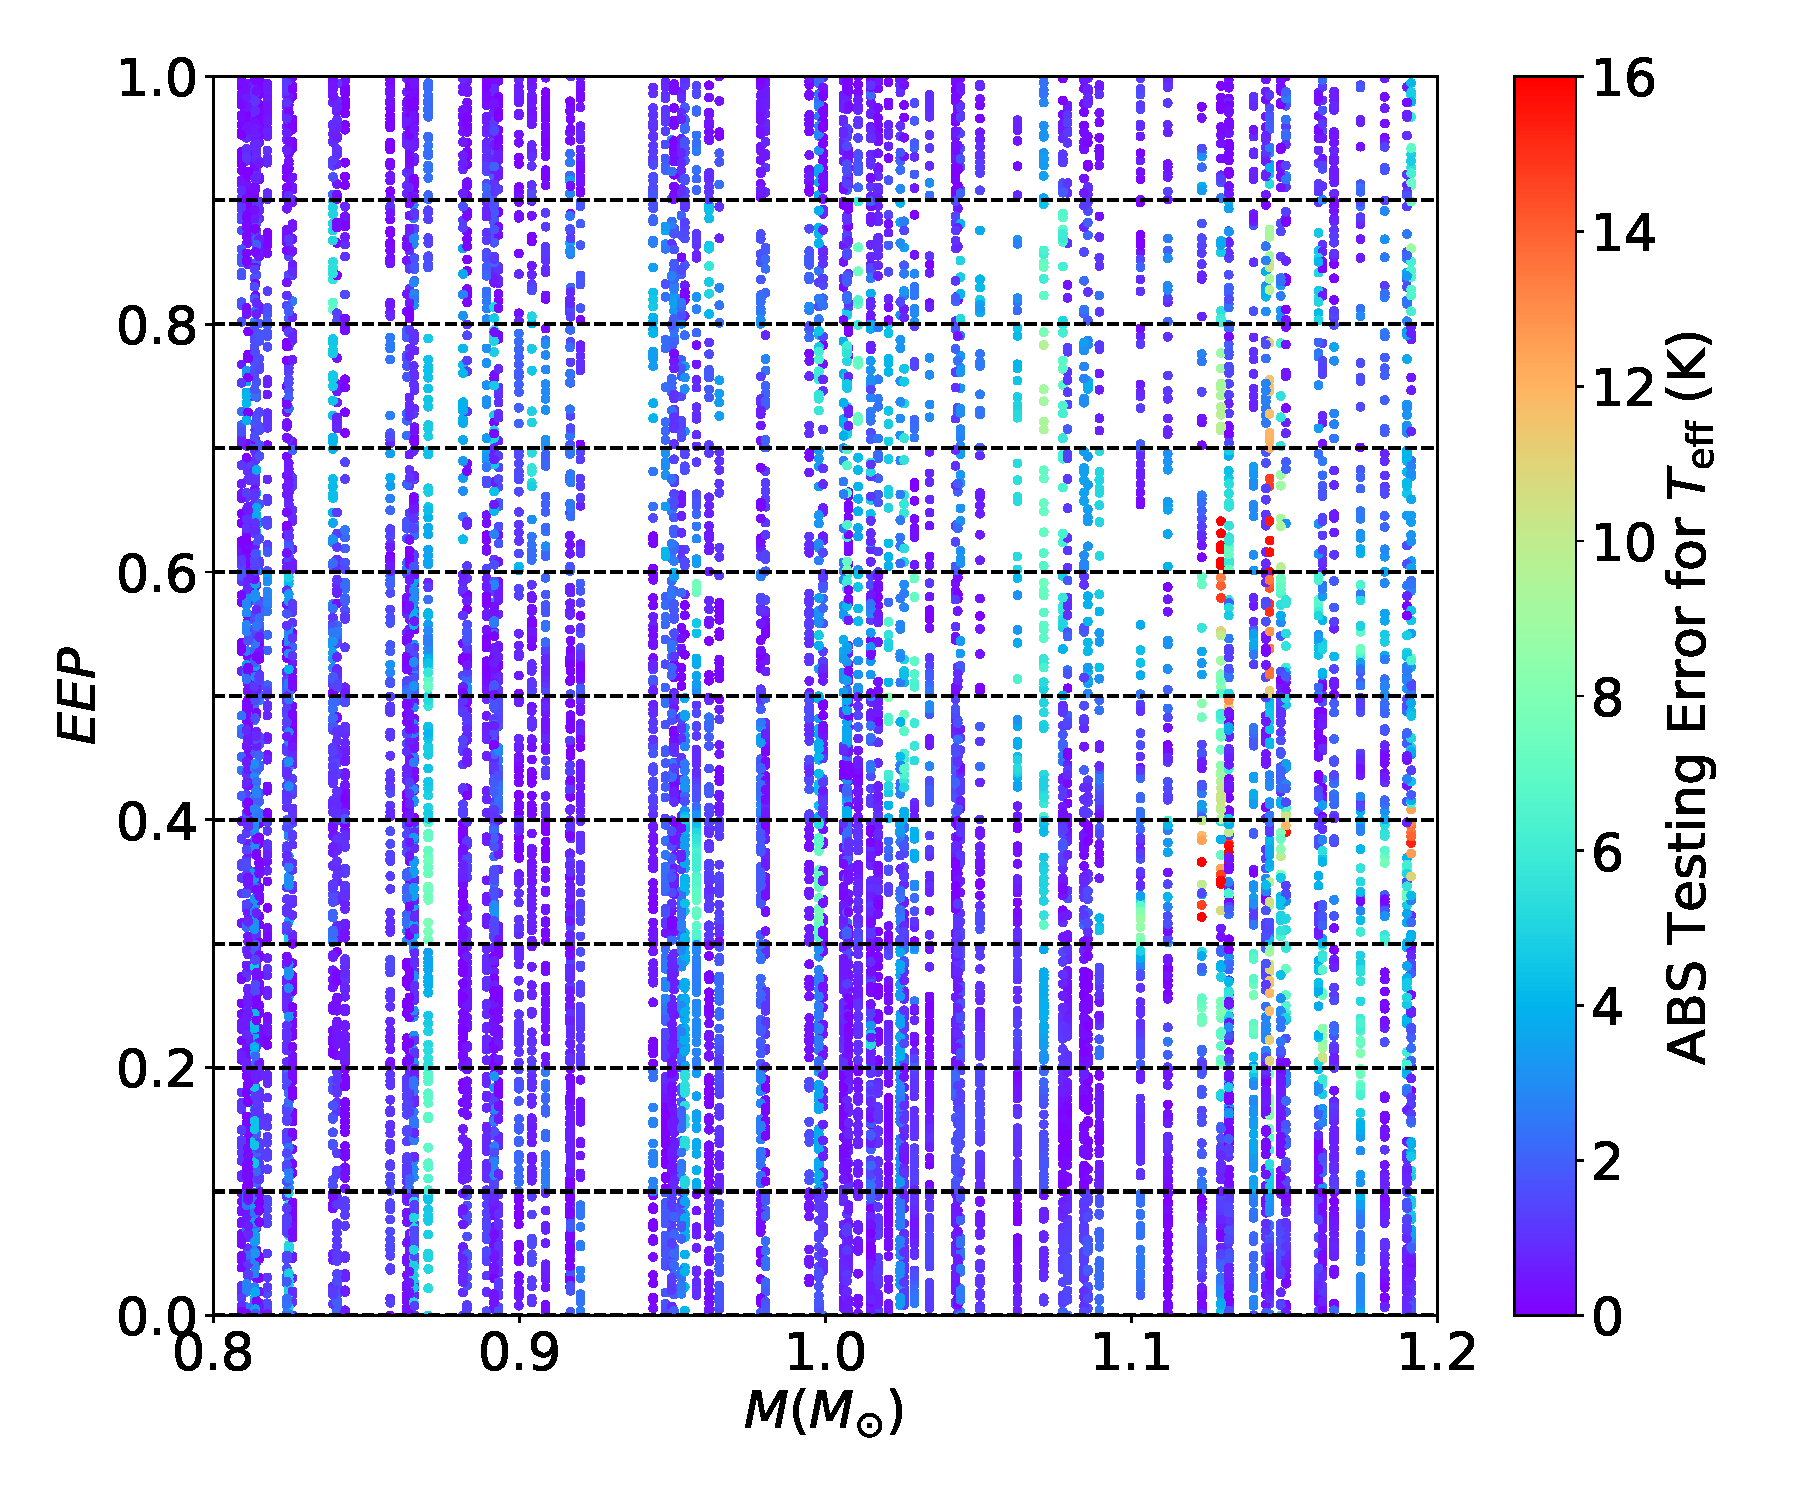
\includegraphics[width=1.0\columnwidth]{3d-testing_teff-10sections.pdf}
	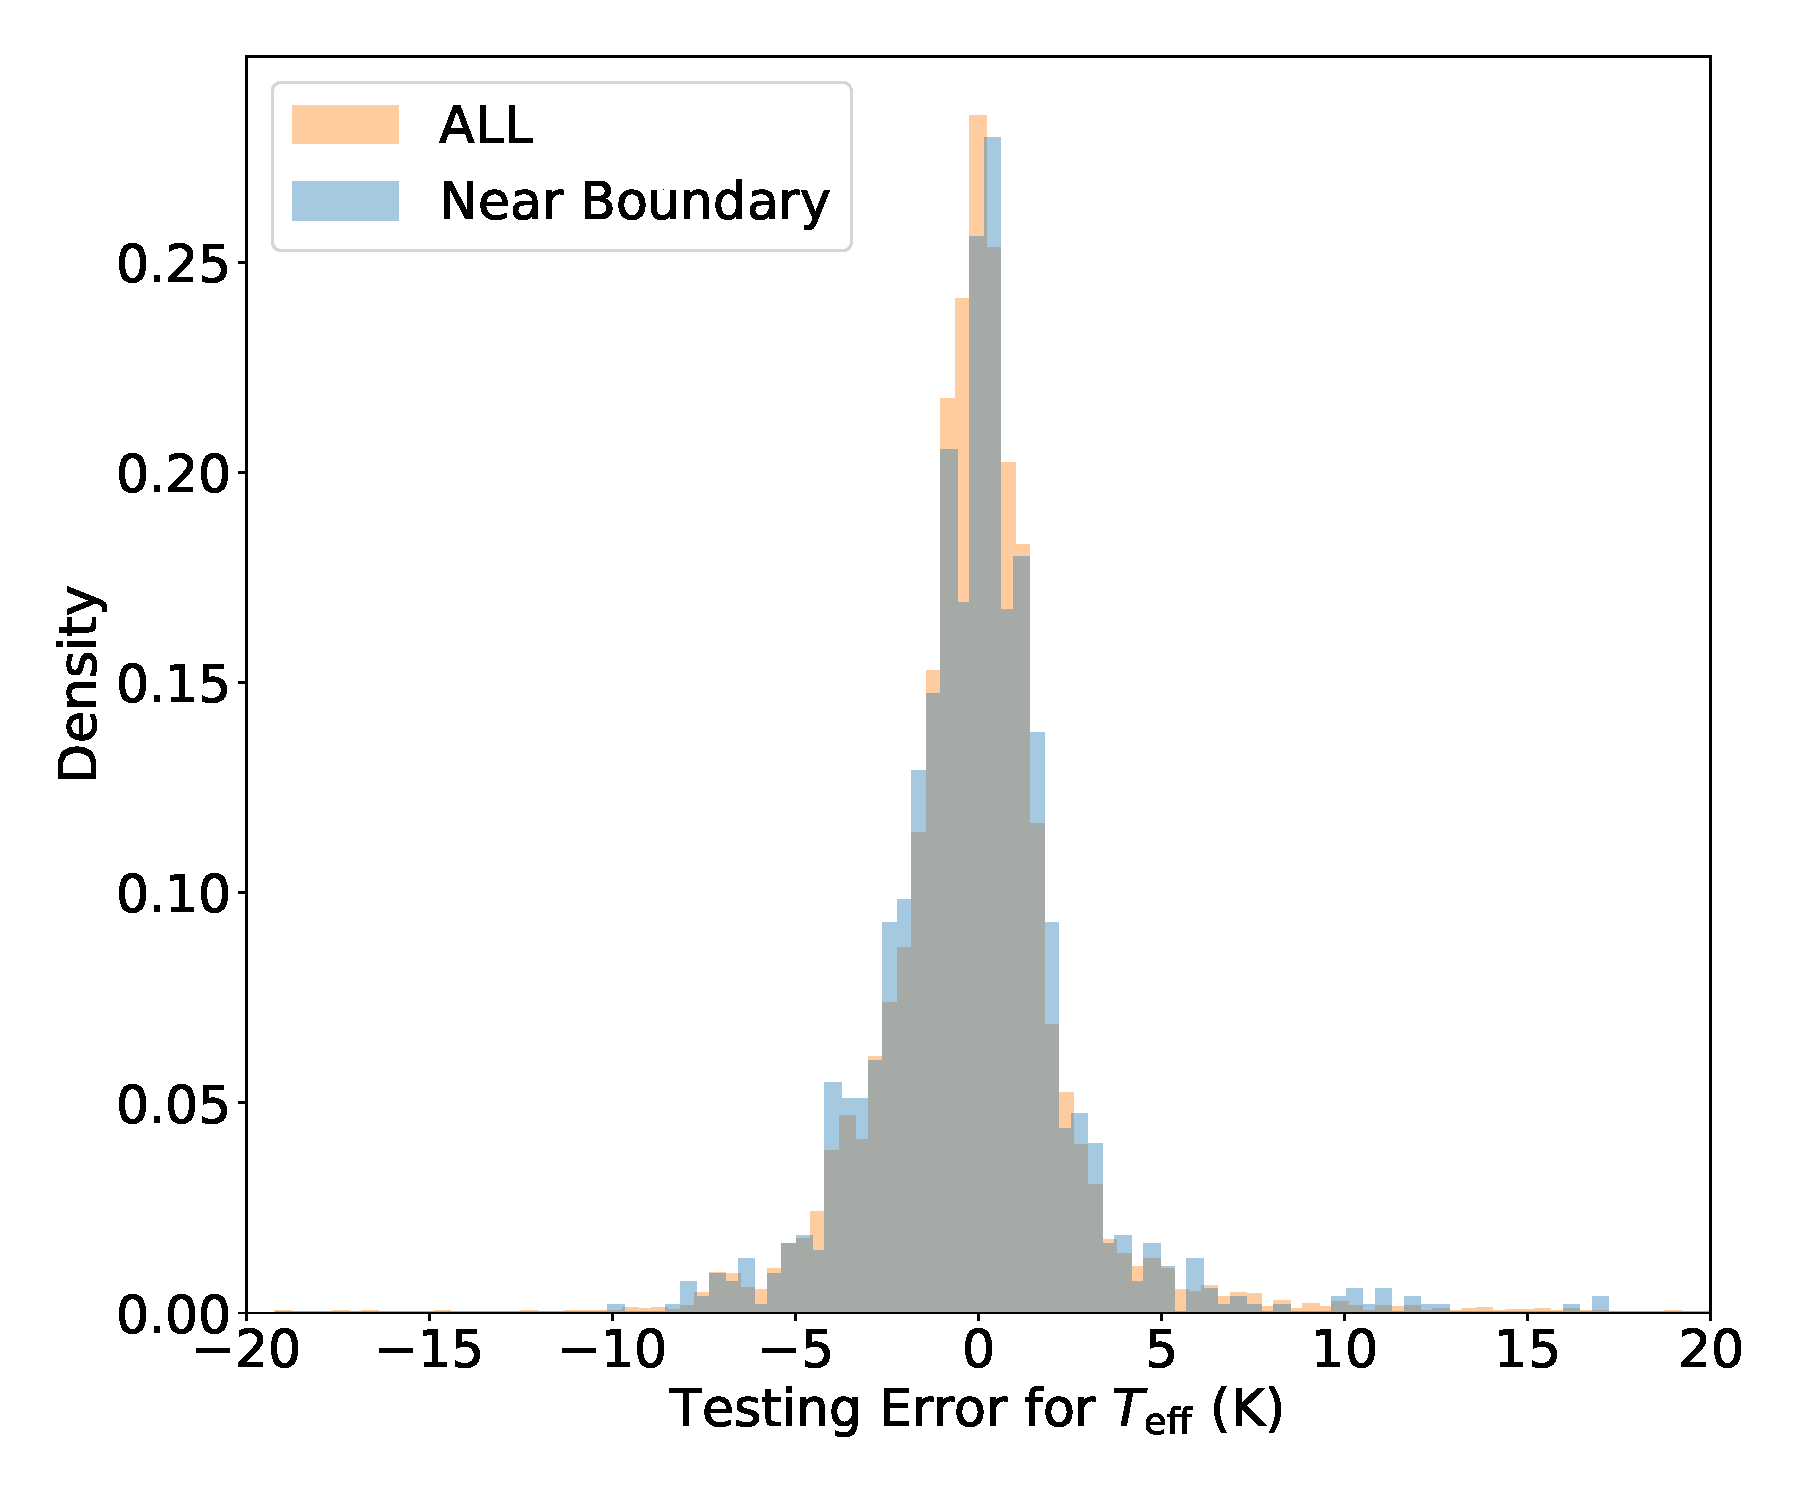
\includegraphics[width=1.0\columnwidth]{3d-testing_teff-hist-10sections.pdf}	
    \caption{Top: Testing errors of 3D GP model for $T_{\rm eff}$ on the $M - EEP$ diagram. Dashes indicates section boundaries. Bottom: examination of the edge effects of the section scenario. Probability distributions of testing errors of all testing data and those near the boundary ($\pm$0.01 EEP) in the upper graph are compared.  As it can be seen, testing errors do not raise around the boundary. }  
    \label{fig:3dtest}
\end{figure}


As mentioned above, the GPU memory captivity limits the actual number of data that induce the kernel function.   
This limitation becomes critical for the high-demission case. To improve, more training data need to be involved. 
%The parameter space exponentially increases with the demission and hence the GP model accuracy inevitable declines. 
%
A simple way is breaking the grid into sections and train GP models for each section separately. 
%The downside of this section scenario is that there will not be one GP model that maps the whole grid. However, as long as the goal of this work is augmenting a model grid but not deriving a universal function for stellar evolutions, this scenario is suitable. 
%Here we test how this section scenario works for 3D GP models. 
Here we divide the training dataset into 10 equal segments by {\it EEP}. We train one \textsc{Exact GP} model with 20,000 training data for each section. 
%We then use the same testing dataset to quantify GP predictions for the five outputs, and 
With this section scenario, the testing EIs for five output parameters are averagely improved by around 10\%. For instance, the testing EI for $T_{\rm eff}$ decreases from 23.5 to 21.6K.
% (1.7/5.0/14.9K at 68/95/99.7\%). 
%

As expected, the section scenario improves the performance of GP model, but there is a major concern about the edge effect at the boundary between sections. If the GP model works significantly poorly at the section boundaries, it will be difficult to map the systematic errors across the whole parameter space. We examine potential edge effects as illustrated in Figure~\ref{fig:3dtest}. We inspect absolute testing errors on the $M-EEP$ diagram. No obvious edge effect is found. We also do a statistical comparison between error values of all data points and those around section boundaries ($\pm0.01EEP$). As shown in the bottom graph, the density distributions of two samples are very similar to each other, indicating no obvious edge effect. We adopt this section scenario to train the stellar grid in the following study.  



